\documentclass{article}


\usepackage[english]{babel} % Language settings 
\usepackage{listings} % Schema Code settings

% Set page size and margins - Replace `letterpaper' with`a4paper' for UK/EU standard size
\usepackage[letterpaper,top=2cm,bottom=2cm,left=3cm,right=3cm,marginparwidth=1.75cm]{geometry}

% Useful packages
\usepackage{amsmath}
\usepackage{graphicx}
\usepackage[colorlinks=true, allcolors=blue]{hyperref}

\usepackage{float}

% title and author of the homework assignment 
\title{CSDS341 Project - Airline Querying System - Initial Report}
\author{Quynh Nguyen (qtn2), Jiamu Zhang (jxz1217), Luke Zhang (rxz330)}

\begin{document}
	
	% set the underline style for schema code
	\lstset{
		language=C, 
		basicstyle=\ttfamily,
		moredelim=[is][\underbar]{-}{-}
	}
	
	\maketitle
	
	\section{Introduction}
	
	\noindent In recent decades, the growing demand for leisure and business travel has led to the prosperity of the airline market. An increasing number of people have been choosing to take flights to travel domestically or internationally. Therefore, an organized and comprehensive database that stores the airline system is critical for both travelers and crew to obtain plenty of simultaneous information.\\
	
	\noindent Although there do exist several flight databases or applications for commercial airlines, it is rare to find comprehensive information - including weather at the departure airport and destination, aircraft type, the total flight hours of pilots, and the number of luggage allowed - in just one database. This information offers travelers a chance to be better prepared for traveling.\\
	
	\noindent Since our airline querying system contains a relatively extensive data sets, the crew members who choose to use our database are able to access the basic information about the travelers who will be on their flight and provides updates about the airline information. 	
	
	\section{Entity-Relationship Model}
	
	\subsection{Assumptions}
	{Before performing the high-level design of the airline querying system, our group lists the following assumptions that need to be considered in our database systems.}
	
	\begin{enumerate}
		\item Assume that there have and only have two types of users of the airline querying system: travelers and crew.
		
		\item Assume that plane ticket information is stored in the database system and each ticket is only valid for one traveler. However, a traveler may own zero or more plane tickets. This matches the real situation in which travelers need to transfer their flights. 
		
		\item Assume that each ticket contains a specific seat location for exactly one flight. However, a flight may have multiple tickets being sold to travelers since a flight has obviously more than one seat.   
		
		\item Assume that a crew member can be either an air attendant or a pilot. Therefore, a crew member can serve zero or more flights. Additionally, a flight must be served by at least one crew member. It does have a slight chance that a small propeller airplane only needs one crew member (i.e. the pilot).
		
		\item Assume that a flight is operated by exactly one aeroplane. For example, figure 1 shows that the aircraft with registration number B-6075 is operating a specific flight (flight number: CA862) from Beijing(PEK) to Geneva(GVA). However, it is likely that one aeroplane can fly multiple flights. It is worth noticing that the  registration number is unique for each aeroplane.
		
		\item Assume that an aeroplane can only belong to one company. This database system does not consider private aeroplanes that do not belong to any company. For instance, the aeroplane B-6075 belongs to Air China. Additionally, a airline company can have multiple planes. 
		
		\item Assume that each airline company must have at least one airport as its hub, a place where the headquarter of the company locates and where the aeroplanes get maintenance and repaired. However, some large airports can provide services for multiple airline companies. For example, Los Angeles International Airport (LAX) is a hub for both United and Delta Airlines, and Delta Airlines has another hub : Detroit Metropolitan Airport (DTW).
		
		\item Assume that each flight can have multiple schedules, and a schedule can be mapped to multiple flights. It is common for most domestic flights to have the same flight flying the same route on two successive days. There is also a slight chance that two flights have the exact same schedule. Additionally, each schedule should have unique \texttt{schedule\_id}.
		
		\item Assume that each flight only departures from exactly one airport and only arrives at exactly one airport. However, an airport can have many flights.
		
		\begin{figure}[H]
			\centering
			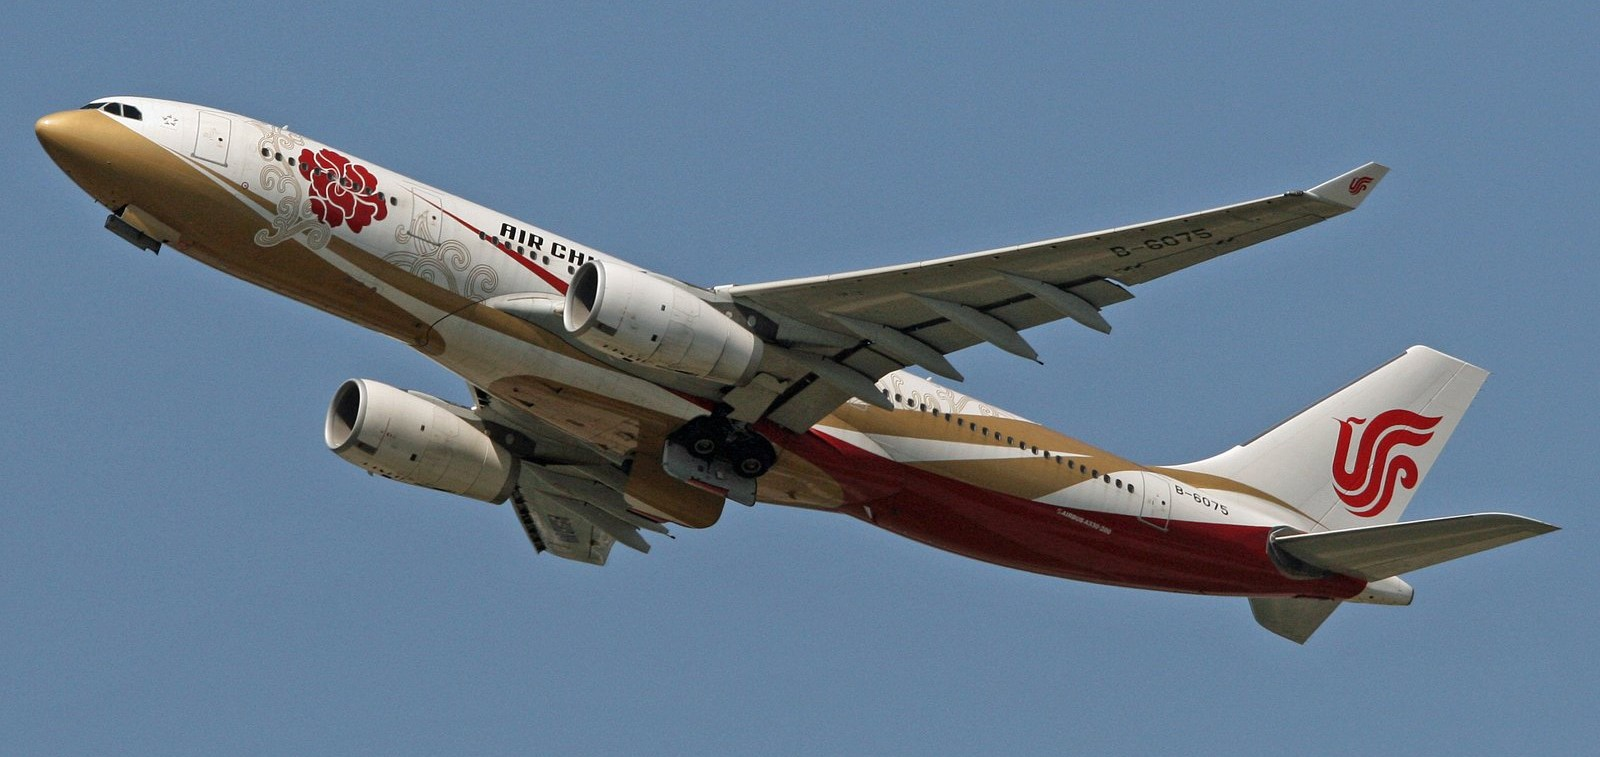
\includegraphics[width=100mm]{CSDS341_Project_B-6075.jpg}
			\caption{Aircraft with Registration Number B-6075 (\copyright Pascal Simon)}
		\end{figure}
		
	\end{enumerate}
	
	\subsection{ER Diagram}
	
	\begin{figure}[H]
		\centering
		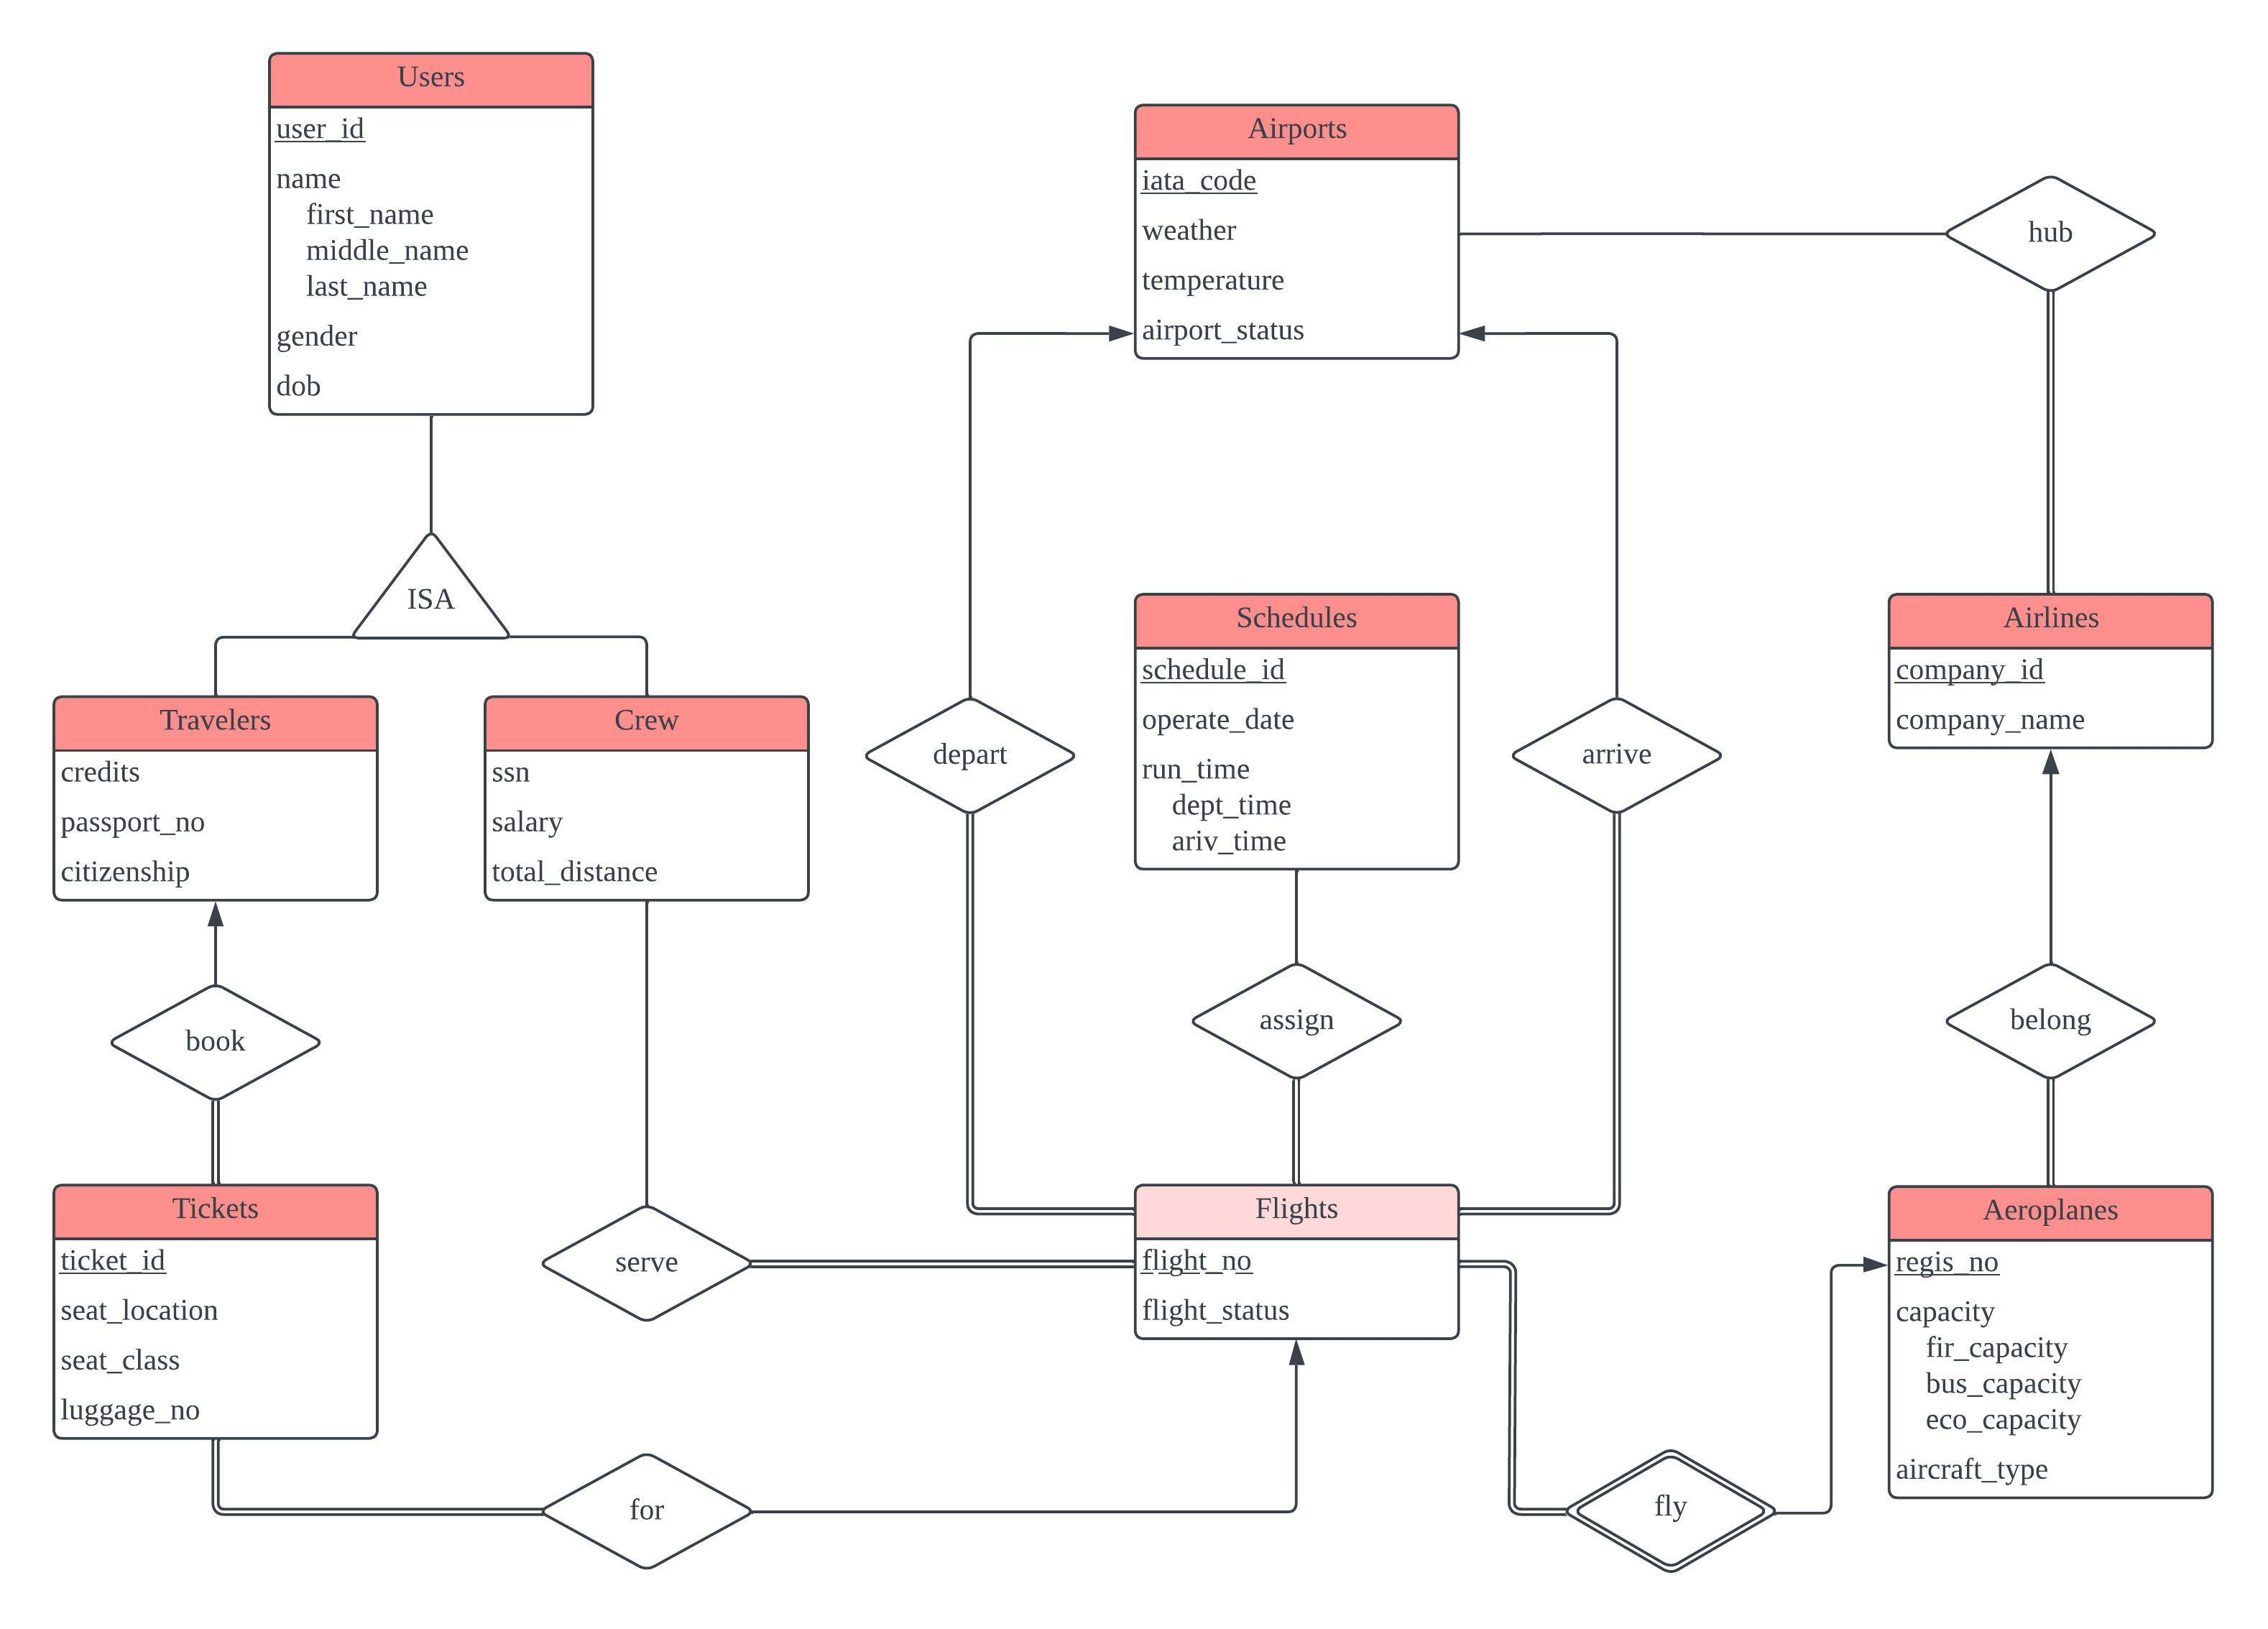
\includegraphics[width=140mm]{CSDS341_Project_ER_Diagram.jpeg}
		\caption{ER Diagram for Airline Querying System}
	\end{figure}
	
	\section{Schemas}
	
	\subsection{Strong Entities}
	
	% Entity: Travelers --------------------------------------------------------
	\noindent The entity \texttt{Travelers} is a type of \texttt{Users} in this Airline Querying Systems. The \texttt{user\_id} attribute is the primary key of this entity.
	\begin{lstlisting}[keepspaces=true]
Travelers(-user_id: int-,
          first_name: varchar(50),
          middle_name: varchar(50),
          last_name: varchar(50),
          gender: char(1),
          dob: date,
          credits: int,
          passport_no: varchar(20), 
          citizenship: varchar(30)
          )
	\end{lstlisting}
    
    % Entity: Crew -------------------------------------------------------------
	\noindent The entity \texttt{Crew} is the other type of \texttt{Users} in this Airline Querying Systems. The \texttt{user\_id} attribute is the primary key of this entity.
	\begin{lstlisting}[keepspaces=true]
Crew(-user_id: int-,
     first_name: varchar(50),
     middle_name: varchar(50),
     last_name: varchar(50),
     gender: char(1),
     dob: date,
     ssn: int, 
     salary: double, 
     total_distance: int
     )
	\end{lstlisting}    

	% Entity: Tickets; Relationship: book & for --------------------------------
	\noindent The table \texttt{Tickets\_book\_for} stores the ticket information of each traveler. The primary key of the entity is  \texttt{ticket\_id}. Since both the \texttt{book} and \texttt{for} relationships are one-to-many relationships, they are merged with the entity on many side which is \texttt{Tickets}. Therefore, there are three different foreign keys in the table. \texttt{traveler\_id} comes from the one side of the \texttt{book} relationship, while \texttt{regis\_no} and \texttt{flight\_no} comes from the one side of the \texttt{for} relationship.

	\begin{lstlisting}[keepspaces=true]
Tickets_book_for(-ticket_id: int-, 
                 seat_location: char(3),
                 seat_class: char(1),
                 luggage_no: int, 
                 traveler_id: int, 
                 regis_no: int,
                 flight_no: varchar(7)
                 )
                 Foreign Key (traveler_id) references (Travelers.user_id)
                 Foreign Key (regis_no) references (Aeroplanes_belong.regis_no)
                 Foreign Key (flight_no) references (Flights_ariv_dept.flight_no)
	\end{lstlisting} 

	% Entity: Airports ---------------------------------------------------------
	\noindent The entity \texttt{Airports} stores the information of airports, with a primary key \texttt{iata\_code}. IATA Code stands for International Air Transport Association Code. It is a three-character code that is unique for each airport. For example, the IATA Code for Los Angeles International Airport is LAX.
	
	\begin{lstlisting}[keepspaces=true]
Airports(-iata_code: char(3)-, 
         weather: varchar(15),
         temperature: int,
         airport_status: varchar(10)
         )
	\end{lstlisting}

	% Entity: Airlines ---------------------------------------------------------
	\noindent The entity \texttt{Airlines} stores the information of airline companies, with a primary key \texttt{company\_id}.
	
	\begin{lstlisting}[keepspaces=true]             
Airlines(-company_id: int-,
         company_name: varchar(30)
         )
	\end{lstlisting}    

	% Entity: Aeroplanes; Relationship: belong ---------------------------------
	\noindent The entity \texttt{Aeroplanes\_belong} stores the information of each aeroplane and the airline company they belong to, with a primary key \texttt{regis\_no} (registration number). Before each plane starts operating, it will be assigned a unique registration number.
	
	\begin{lstlisting}[keepspaces=true]               
Aeroplanes_belong(-regis_no: varchar(10)-,
                  fir_capacity: int,
                  bus_capacity: int, 
                  eco_capacity: int,
                  aircraft_type: varchar(10), 
                  company_id: int
                  )
                  Foreign Key (company_id) references (Airlines.company_id)
	\end{lstlisting}    
	
	% Entity: Schedules --------------------------------------------------------
	\noindent The entity \texttt{Schedules} stores the flight schedules. The primary key is \texttt{schedule\_id}.
	\begin{lstlisting}[keepspaces=true] 
Schedules(-schedule_id: int-, 
          operate_date: date,
          dept_time: time,
          ariv_time: time
          )
	\end{lstlisting}

	\subsection{Weak Entities}
	
	% Weak Entity: Flights; Id relationship: fly; Relationship: ariv dept------
	\noindent The weak entity \texttt{Flights\_ariv\_dept} stores the information of each flight operated by each aeroplane and the \texttt{depart} \& \texttt{arrive} information. The primary key of the weak entity is \texttt{regis\_no} and \texttt{flight\_no}. It contains foreign keys obtains from both \texttt{Aeroplanes} and \texttt{Airports} Entities. This table merges the weak entity \texttt{Flights}, the identifying relationship \texttt{fly} and two many to one relationships (\texttt{depart} and \texttt{arrive}). 
	\begin{lstlisting}[keepspaces=true]        
Flights_ariv_dept(-regis_no: int-, 
                  -flight_no: varchar(7)-,
                  flight_status: varchar(10),
                  dept_iata_code: char(3),
                  ariv_iata_code: char(3)
                  )
                  Foreign Key (regis_no) references (Aeroplanes_belong.regis_no)
                  Foreign Key (dept_iata_code) references (Airports.iata_code)
                  Foreign Key (ariv_iata_code) references (Airports.iata_code)
	\end{lstlisting}

	\subsection{Relationships}
	
	\noindent The \texttt{book} relationship is merged with the entity \texttt{Tickets} in the table \texttt{Tickets\_book\_for}. \\
	
	\noindent The \texttt{for} relationship is merged with the entity \texttt{Tickets} in the table \texttt{Tickets\_book\_for}. \\
	
	\noindent The \texttt{dept} relationship is merged with the entity \texttt{Flights} in the table \texttt{Flights\_ariv\_dept}. \\
	
	\noindent The \texttt{ariv} relationship is merged with the entity \texttt{Flights} in the table \texttt{Flights\_ariv\_dept}. \\
	
	\noindent The \texttt{belong} relationship is merged with the entity \texttt{Aeroplanes} in the table \texttt{Aeroplanes\_belong}. \\
	
	% Relationsip: serve -------------------------------------------------------
	\noindent The \texttt{serve} relationship stores the information regarding how crew members serve for flights. Since each crew member can serve multiple flights and a flight may need multiple crews, this is a many-to-many relationship. Therefore, the primary keys from both sides should be set as the primary keys of this relationship.
	\begin{lstlisting}[keepspaces=true]        
serve(-crew_id: int-, 
      -regis_no: int-, 
      -flight_no: varchar(7)-
      )
      Foreign Key (crew_id) references (Crew.user_id)
      Foreign Key (regis_no) references (Aeroplanes_belong.regis_no)
      Foreign Key (flight_no) references (Flights_ariv_dept.flight_no)
	\end{lstlisting}    

	% Relationship: assign -----------------------------------------------------
	\noindent The \texttt{assign} relationship stores the information regarding the mapping between flights and schedules. Since this is a many-to-many relationship, the primary keys from both sides should be set as the primary keys of this relationship.
	\begin{lstlisting}[keepspaces=true]		
assign(-regis_no: varchar(10)-,
       -flight_no: varchar(7)-,
       -schedule_id: int-
       )
       Foreign Key (regis_no) references (Aeroplanes_belong.regis_no)
       Foreign Key (flight_no) references (Flights_ariv_dept.flight_no)
       Foreign Key (schedule_id) references (Schedules.schedule_id)
	\end{lstlisting}    
	
	% Relationship: hub --------------------------------------------------------
	\noindent The \texttt{hub} relationship stores the information regarding airline companies and their hub airports. Since this is a many-to-many relationship, the primary keys from both sides should be set as the primary keys of this relationship.
	\begin{lstlisting}[keepspaces=true]	
hub(-company_id: int-,
    -iata_code: char(3)-
    )
    Foreign Key (company_id) references (Airlines.company_id)
    Foreign Key (iata_code) references (Airports.iata_code)
	\end{lstlisting}    
	
	\subsection{Identifying Relationships}
	
	All the identifying relationships in the schema are merged with the weak entity. There is no need to create separate tables because that may cause redundancies.
	
	\section{Example Queries}
	
	\noindent Find the passport number of all Chinese Traveler who has already booked at least one Plane Ticket. 
	% query starts here
	\begin{verbatim}
		SELECT    passport_no 
		FROM      Travelers
		WHERE     (Citizenship = "Chinese") 
		          AND 
		          (user_id IN (SELECT    traveler_id, count(ticket_id)
		                       FROM      Tickets_book_for
		                       GROUP BY  traveler_id
		                       HAVING    count(ticket_id) >= 1));
	\end{verbatim}
    % query ends here
    
	\noindent Find the flight number of all flights that belongs to \textit{Emirates} and has over 30-seat capacity in first class. 
	% query starts here
	\begin{verbatim}
		SELECT    flight_no
		FROM      Flights_ariv_dept NATURAL JOIN Aeroplanes_belongs
		WHERE     (Aeroplanes_belongs.fir_capacity > 30) 
		          AND
		          (regis_no IN (SELECT    regis_no
		                        FROM      Aeroplanes_belongs NATURAL JOIN Airlines
		                        WHERE     Airlines.company_name = "Emirates"))               
	\end{verbatim}
	% query ends here
	
	\noindent Find the flight number of all flights that departs from Los Angeles International Airport on both 2021-06-22 and 2021-06-23.
	% query starts here
	\begin{verbatim}
		SELECT flight_no
		FROM   Flights_ariv_dept
		WHERE  (dept_iata_code = "LAX")
		       AND 
		       (flight_no IN (SELECT flight_no
		                      FROM   Flights_ariv_dept NATURAL JOIN assign NATURAL JOIN Schedules AS s22
		                      WHERE  s22.operate_date = "2021-06-22"
		                             AND
		                             (exists(SELECT flight_no
		                                     FROM   Flights_ariv_dept NATURAL JOIN assign 
		                                            NATURAL JOIN Schedules AS s23
		                                     WHERE  s23.operate_date = "2021-06-23"
		                                            AND
		                                            s22.flight_no = s23.flight_no))))     
	\end{verbatim}
	% query ends here
	
	\section{Data Sources}
	Since there exists various sources about flight numbers and their departure or arrival information, we are able to use real data for most flights. However, it is hard to keep track on the real-time temperature or status of the airport. For this part of data, our group decide to use make-up data. For travelers and crew information, since the data are usually protected by the airline companies, we also decide to use make up data. 
	
\end{document}